\documentclass{article}
\usepackage{eason}

\usepackage{pdfpages}

\usepackage[a4paper, margin=1in]{geometry}

\usepackage{lipsum}
\usepackage{mwe}

\usemintedstyle{bw}

\usepackage{titlesec}
\titleformat{\section}{\normalfont\Large\bfseries}{}{0pt}{}

\title{\LaTeX\ Template File}
\author{Eason Shao}

\begin{document}
% \maketitle

{\LARGE\bf 0.1}

\vspace*{-10mm}
\hfill\framebox{\parbox[t][5 true cm][c]{11 true cm}{\hfil
        Space for the project label }}

\bigbreak

\begin{center}\LARGE\bf
    Root Finding in One Dimension
\end{center}

\clearpage

\section{Question 1}

To show the function \(F\pqty{x} = 2x - 3 \sin x + 5\) has exactly one root, it suffices to consider the region \(\ccintv{-4}{-1}\), since:
\begin{itemize}
    \item if \(x < -4\), then \(F\pqty{x} = \pqty{2x + 5} - 3 \sin x < -3 + 3 = 0\); and
    \item if \(x > -1\), then \(F\pqty{x} > 3 - 3 = 0\).
\end{itemize}

Regarranging \(F\pqty{x} = 0\) to \(2x + 5 = 3 \sin x\), \autoref{fig:question-1-fig} plots the functions in the region concerned.

\begin{figure}[ht!]
    \centering
    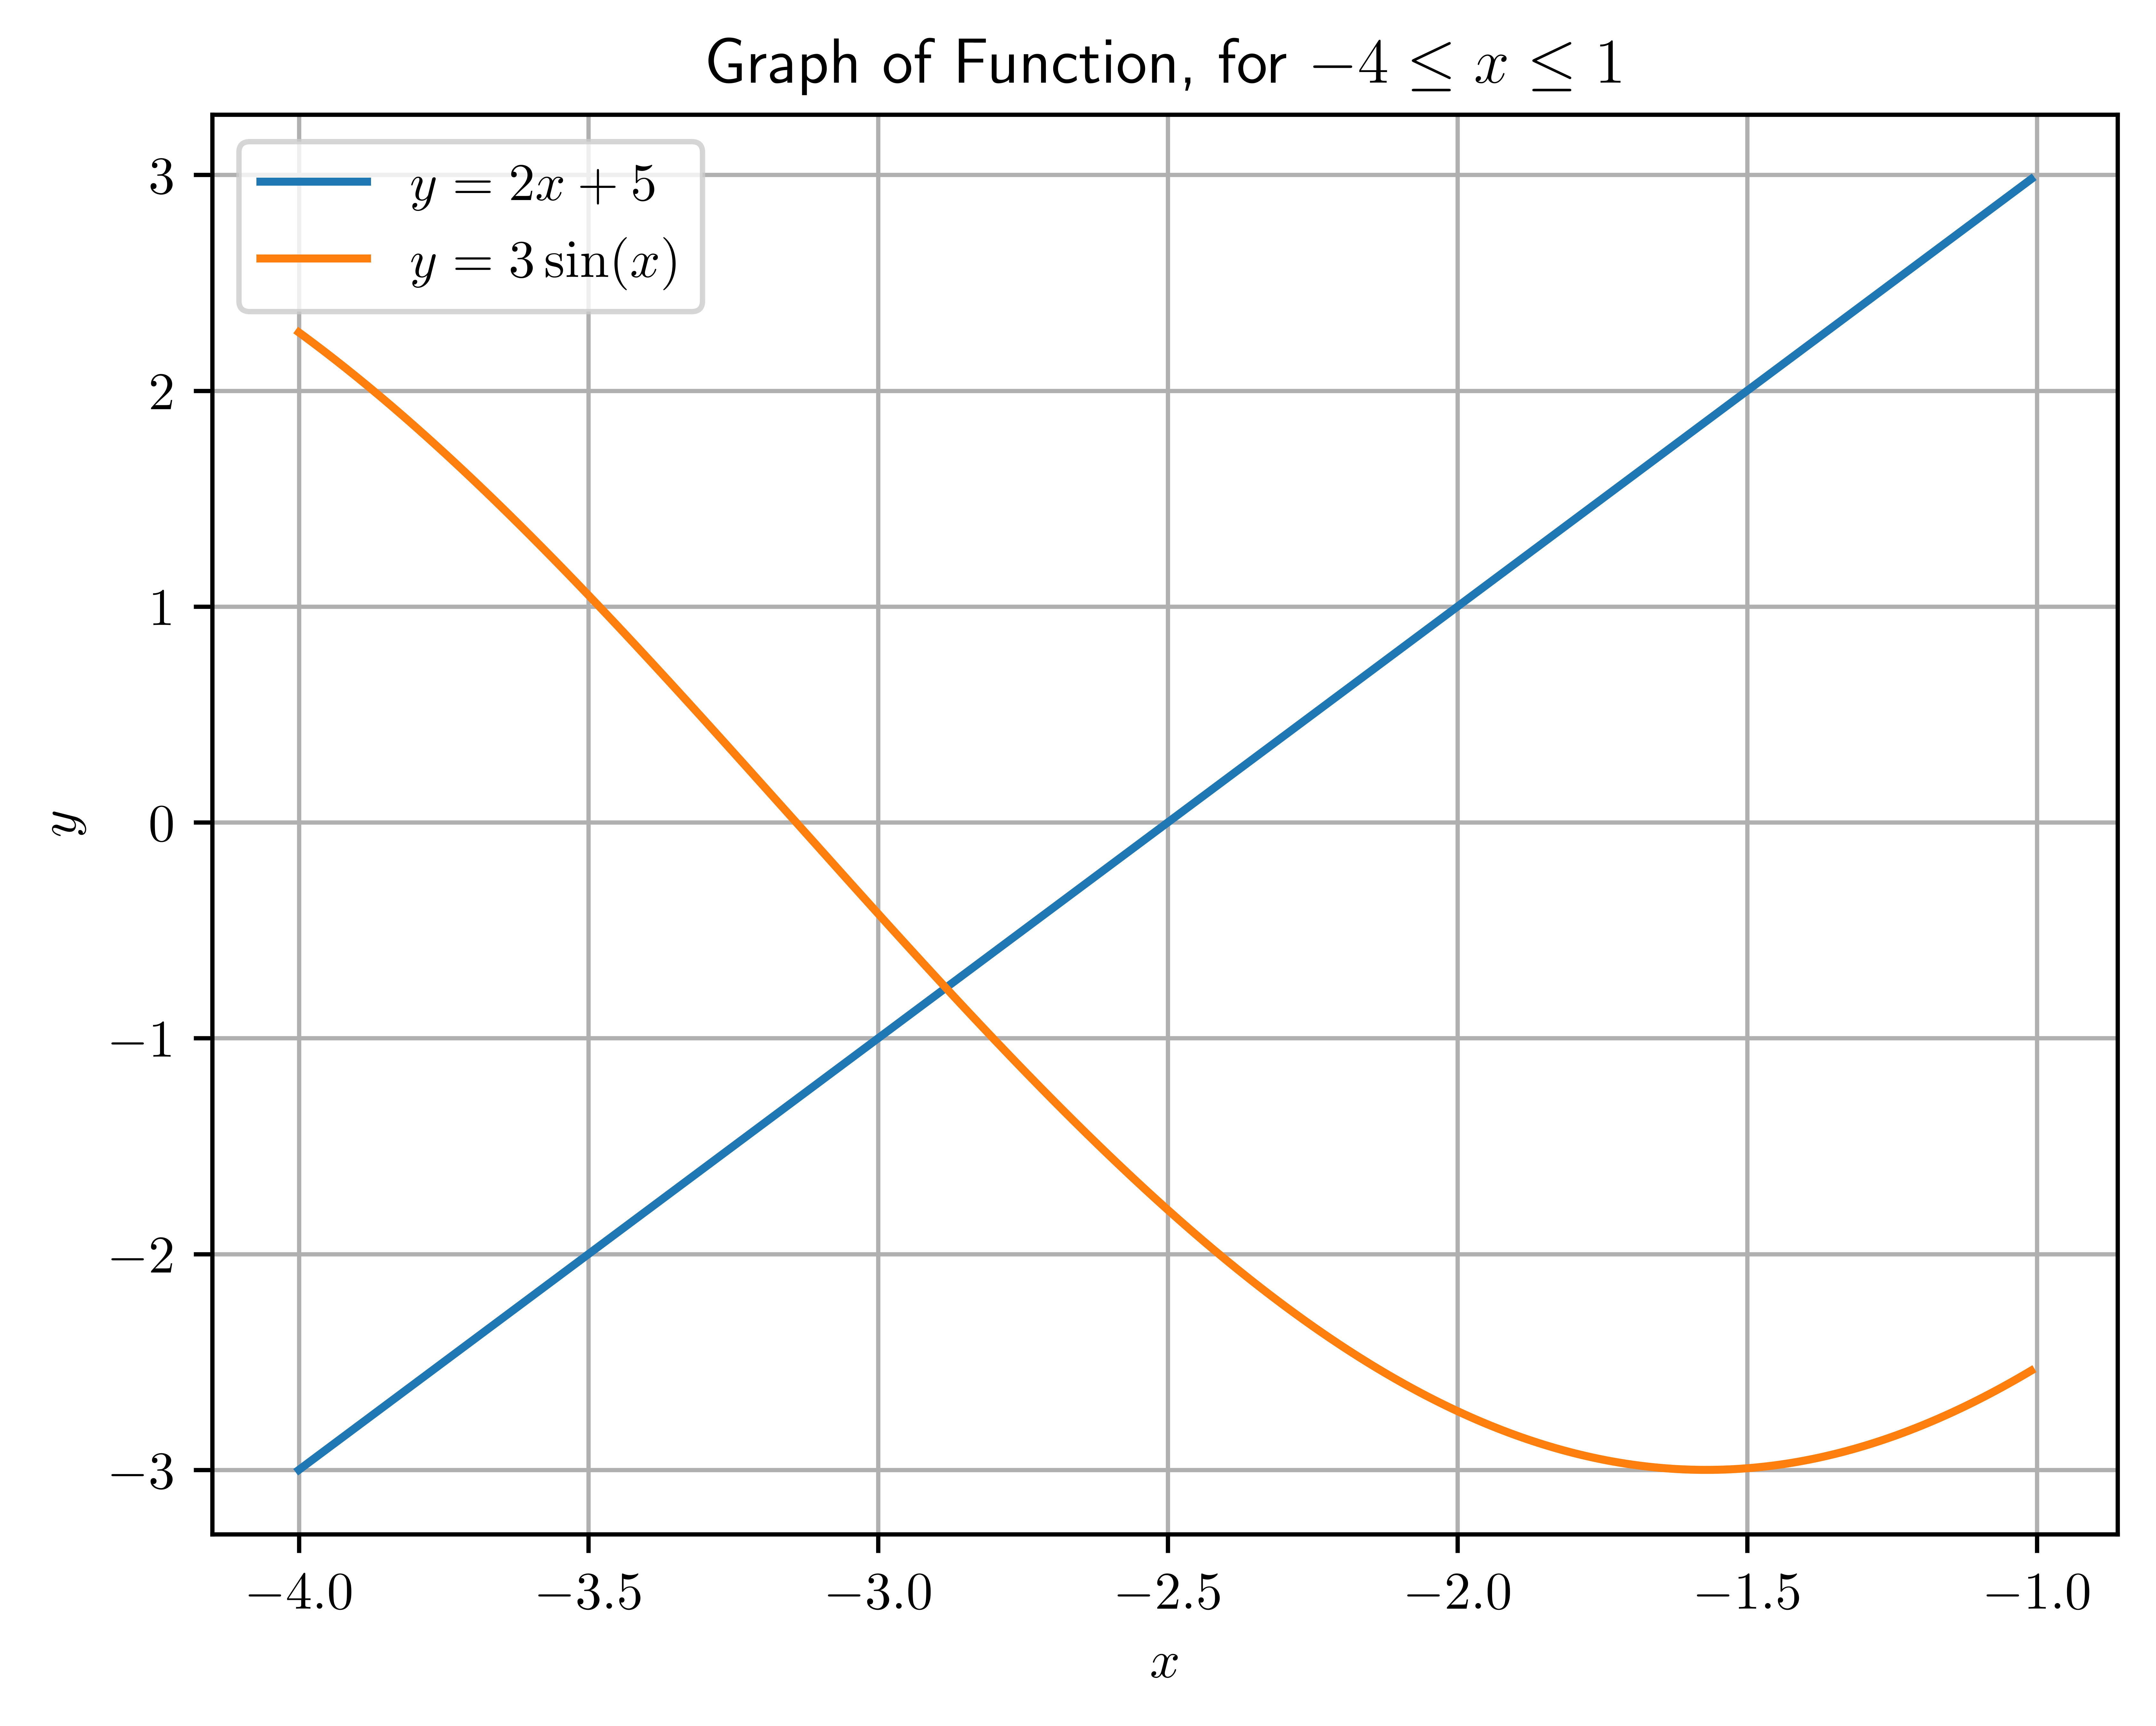
\includegraphics[width=0.8\textwidth]{fig/question-1.png}
    \caption{Graph of Functions, for \(4 \leq x \leq 1\)}
    \label{fig:question-1-fig}%
\end{figure}

The function \(y = 3 \sin x\) is strictly decreasing on \(\ccintv{-\flatfrac{3\pi}{2}}{-\flatfrac{\pi}{2}} \supseteq \ccintv{-4}{-\flatfrac{\pi}{2}}\), and the function \(y = 2x + 5\) is strictly increasing on that interval, so there is precisely one root on that interval. As for \(x \in \ccintv{\flatfrac{-\pi}{2}}{-1}\), note that \(3 \sin x < 0\) on that interval, while \(2x + 5 > 0\), so there cannot be any roots on that interval. 

\section{Programming Task: Binary Search}

The program was ran on suitable starting values, and some results are included in \autoref{tab:programming-task-binary-search}%

\begin{table}[ht!]
    \centering
    \caption{Binary Search Results}
    \smallskip 
    \begin{tabular}{|c|c|c|c|}
        \hline
        Initial Endpoints & Iterations & Final Value & Truncation Error \\
        \hline
        \(\ccintv{-3}{-2}\) & \(17\) & \(-2.8832359\ldots\) & \(\num{\pm 3.8146e-6}\) \\
        \(\ccintv{-\pi}{0}\) & \(19\) & \(-2.8832397\ldots\) & \(\num{\pm 2.9960e-6}\) \\
        \(\ccintv{-10}{10}\) & \(19\) & \(-2.8832368\ldots\) & \(\num{\pm 2.8610e-6}\) \\
        \hline
    \end{tabular}
    \label{tab:programming-task-binary-search}
\end{table}

\section{Question 2}

Suppose after the final binary search iteration, we end up in the interval \(\ccintv{a}{b}\), where the computed values of \(F\pqty{a}\) and \(F\pqty{b}\) satisfy \(F_c\pqty{a} < 0\) and \(F_c\pqty{b} > 0\), and by the requirement of truncation value that \(\flatfrac{\pqty{b - a}}{2} < \num{0.5e-5}\).

If we have \(F_c\pqty{a} < - \delta\) and \(F_c\pqty{b} > \delta\), then \(F\pqty{a} < 0\) and \(F\pqty{b} > 0\), meaning our root must lie in the interval we claimed.

If not, say \(-\delta < F_c\pqty{a} < 0\), then we must have \(-2 \delta < F\pqty{a} < \delta\). Suppose if \(F\pqty{a}\) is of the other sign, i.e., \(0 < F \pqty{a} < \delta\), then its actual value must satisfy, by Taylor's theorem
\begin{equation}
    F\pqty{a} \approx F'\pqty{x_{\ast}} \pqty{a - x_{\ast}}
\end{equation}
and hence rearranging gives
\begin{equation}
    \abs{a - x_{\ast}} \approx \abs{\frac{F\pqty{a}}{F'\pqty{x_{\ast}}}} < \frac{\delta}{4}
\end{equation}
by the hint of \(\abs{F'\pqty{x}} > 4\) and that \(x_{\ast} \in \oointv{-\flatfrac{\pi}{4}}{\flatfrac{-3\pi}{4}}\). Hence, in this case, the accuracy will be approximately
\begin{equation}
    \num{0.5e-5} + \frac{\delta}{4}.
\end{equation}

\section{Programming Task: Fixed-Point Iteration}

\section{Question 3}

\paragraph{i. Divergence} \autoref{fig:question-3-i} gives the iteration process (in green) when we use the initial values specified in (i). Notice that the iteration values oscillates between approximately \(-4.0\) and approximately \(-1.4\), and in particular, never converges.

\begin{figure}[ht!]
    \centering
    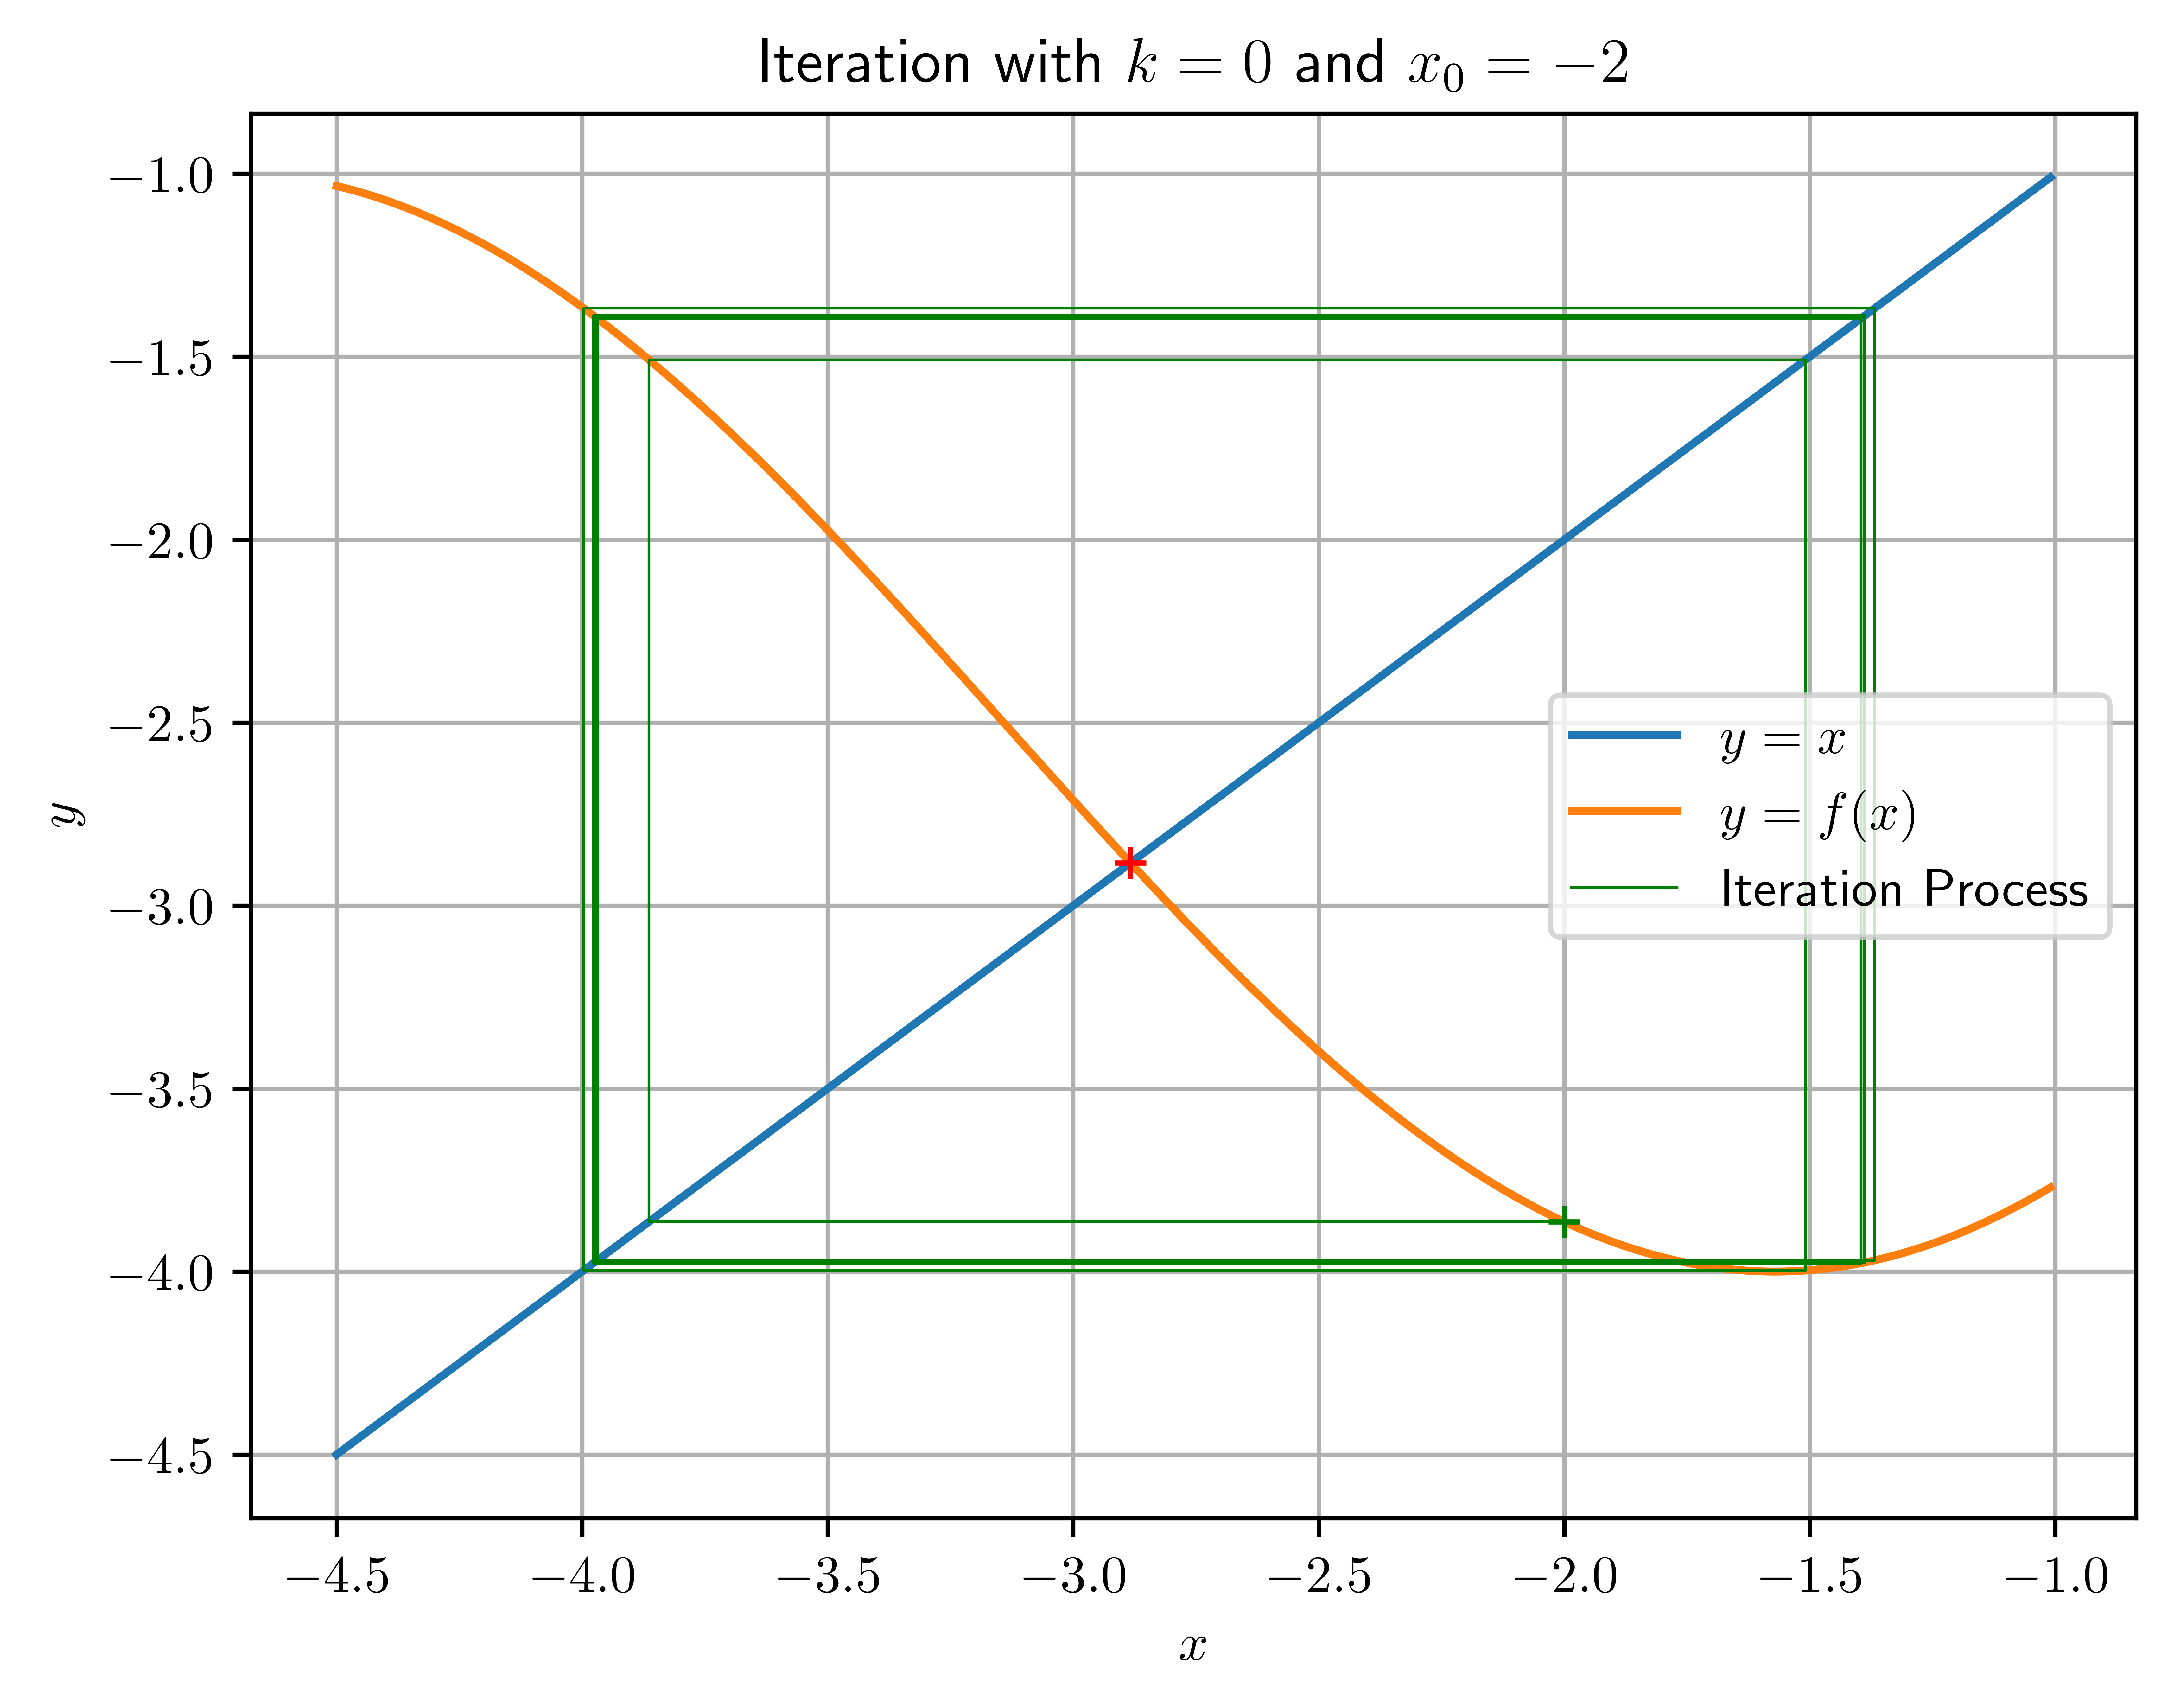
\includegraphics[width=0.8\textwidth]{fig/question-3-i.png}
    \caption{Iteration Process with \(k = 0\) and \(x_0 = -2\)}
    \label{fig:question-3-i}%
\end{figure}

Mathematically speaking, divergence occurs because of the following. Let \(x_{\ast}\) be a fixed point. Then the iteration satisfies \(f\pqty{x_\ast} = x_\ast\) at the point itself, and for the iteration to converge to the fixed point, if \(x_N\) is near the fixed point, then \(x_{N + 1} = f\pqty{x_N}\), we note
\begin{equation}
    \label{eq:divergence-proof}%
    \begin{aligned}
        x_{N + 1} &= f\pqty{x_N} \\
        &\approx f\pqty{x_{\ast}} + f'\pqty{x_{\ast}} \pqty{x_{N} - x_{\ast}} \\
        &= x_{\ast} + f'\pqty{x_{\ast}} \pqty{x_{N} - x_{\ast}},
    \end{aligned}
\end{equation}
so by rearranging, we have
\begin{equation}
    \label{eq:error-local}%
    \epsilon_{N + 1} \approx f'\pqty{x_{\ast}} \epsilon_{N}
\end{equation}
where \(\epsilon_N = x_N - x_{\ast}\) is the truncation error at the \(N\)-th iteration. It follows that, if \(\abs{f'\pqty{x_{\ast}}} > 1\), then the iteration process cannot converge to the fixed point. For this case where \(k = 0\), note
\begin{equation}
    f'\pqty{x_{\ast}} = \frac{3 \cos x}{2} \approx -1.45021\ldots < -1
\end{equation}
and therefore this iteration process must diverge.

\paragraph{ii. Convergence} Since \(\oointv{-\pi}{-\flatfrac{\pi}{2}}\) is a relatively large interval, we consider the Taylor theorem with the Lagrange reminder, which gives
\begin{equation}
    \label{eq:error-global}%
    \epsilon_{N + 1} = f'\pqty{\xi_N} \epsilon_N
\end{equation}
where \(\xi_N\) lies between \(x_N\) and \(x_{\ast}\) (note that in \autoref{eq:error-local} that this \(\xi_N\) was \(x_{\ast}\)). Therefore, it suffices to have \(f'\pqty{x} \in \oointv{-1}{1}\) for all \(x \in \oointv{-\pi}{-\flatfrac{\pi}{2}}\). We have
\begin{equation}
    f'\pqty{x} = \frac{3 \cos x + k}{2 + k}
\end{equation}
and note that \(\cos\) is increasing in this interval, so therefore this is equivalent to having
\begin{equation}
    f'\pqty{-\pi} = \frac{-3 + k}{2 + k} > -1 \qand f'\pqty{-\frac{\pi}{2}} = \frac{k}{2 + k} < 1,
\end{equation}
the first of which solves to \(\boxed{k > \frac{1}{2}}\), and the second of which always holds given this. Therefore, this is precisely the range of values of \(k\) that convergence is guaranteed.

\paragraph{iii. Monotonic and Oscillatory Convergence} Again, this question concerns the behaviour near the root \(x_{\ast}\), so we recall \autoref{eq:error-local}, and observe that \term{monotonic} convergence corresponds to when \(0 < f'\pqty{x_{\ast}} < 1\) (in which case the error terms have identical signs), and \term{oscillatory} convergence corresponds to when \(-1 < f'\pqty{x_{\ast}} < 1\) (in which case the error terms oscillate between positive and negative).

Choosing \(k = 3\) will give \(f'\pqty{x_{\ast}} > 0\) since \(3 \cos x + 3 \geq 0\), taking equal sign if and only if \(x = \pi + n \pi\) for \(n \in \ZZ\), where \(x_{\ast}\) is certainly not the case. This will give monotonic convergence for a sufficiently good initial guess, and in fact with our initial guess of \(-2\), the program terminates after \(5\) iterations with \(\epsilon = \num{1e-5}\), as plotted in \autoref{fig:question-3-iii-1}.

On the other hand, choosing \(k = 1\) will give \(f'\pqty{x_{\ast}} = -0.63347\ldots < 0\), so we will expect oscillatory convergence for a sufficiently good initial guess, as plotted in \autoref{fig:question-3-iii-2}.


\begin{figure*}[ht!]
    \centering
    \begin{subfigure}[t]{0.5\textwidth}
        \centering
        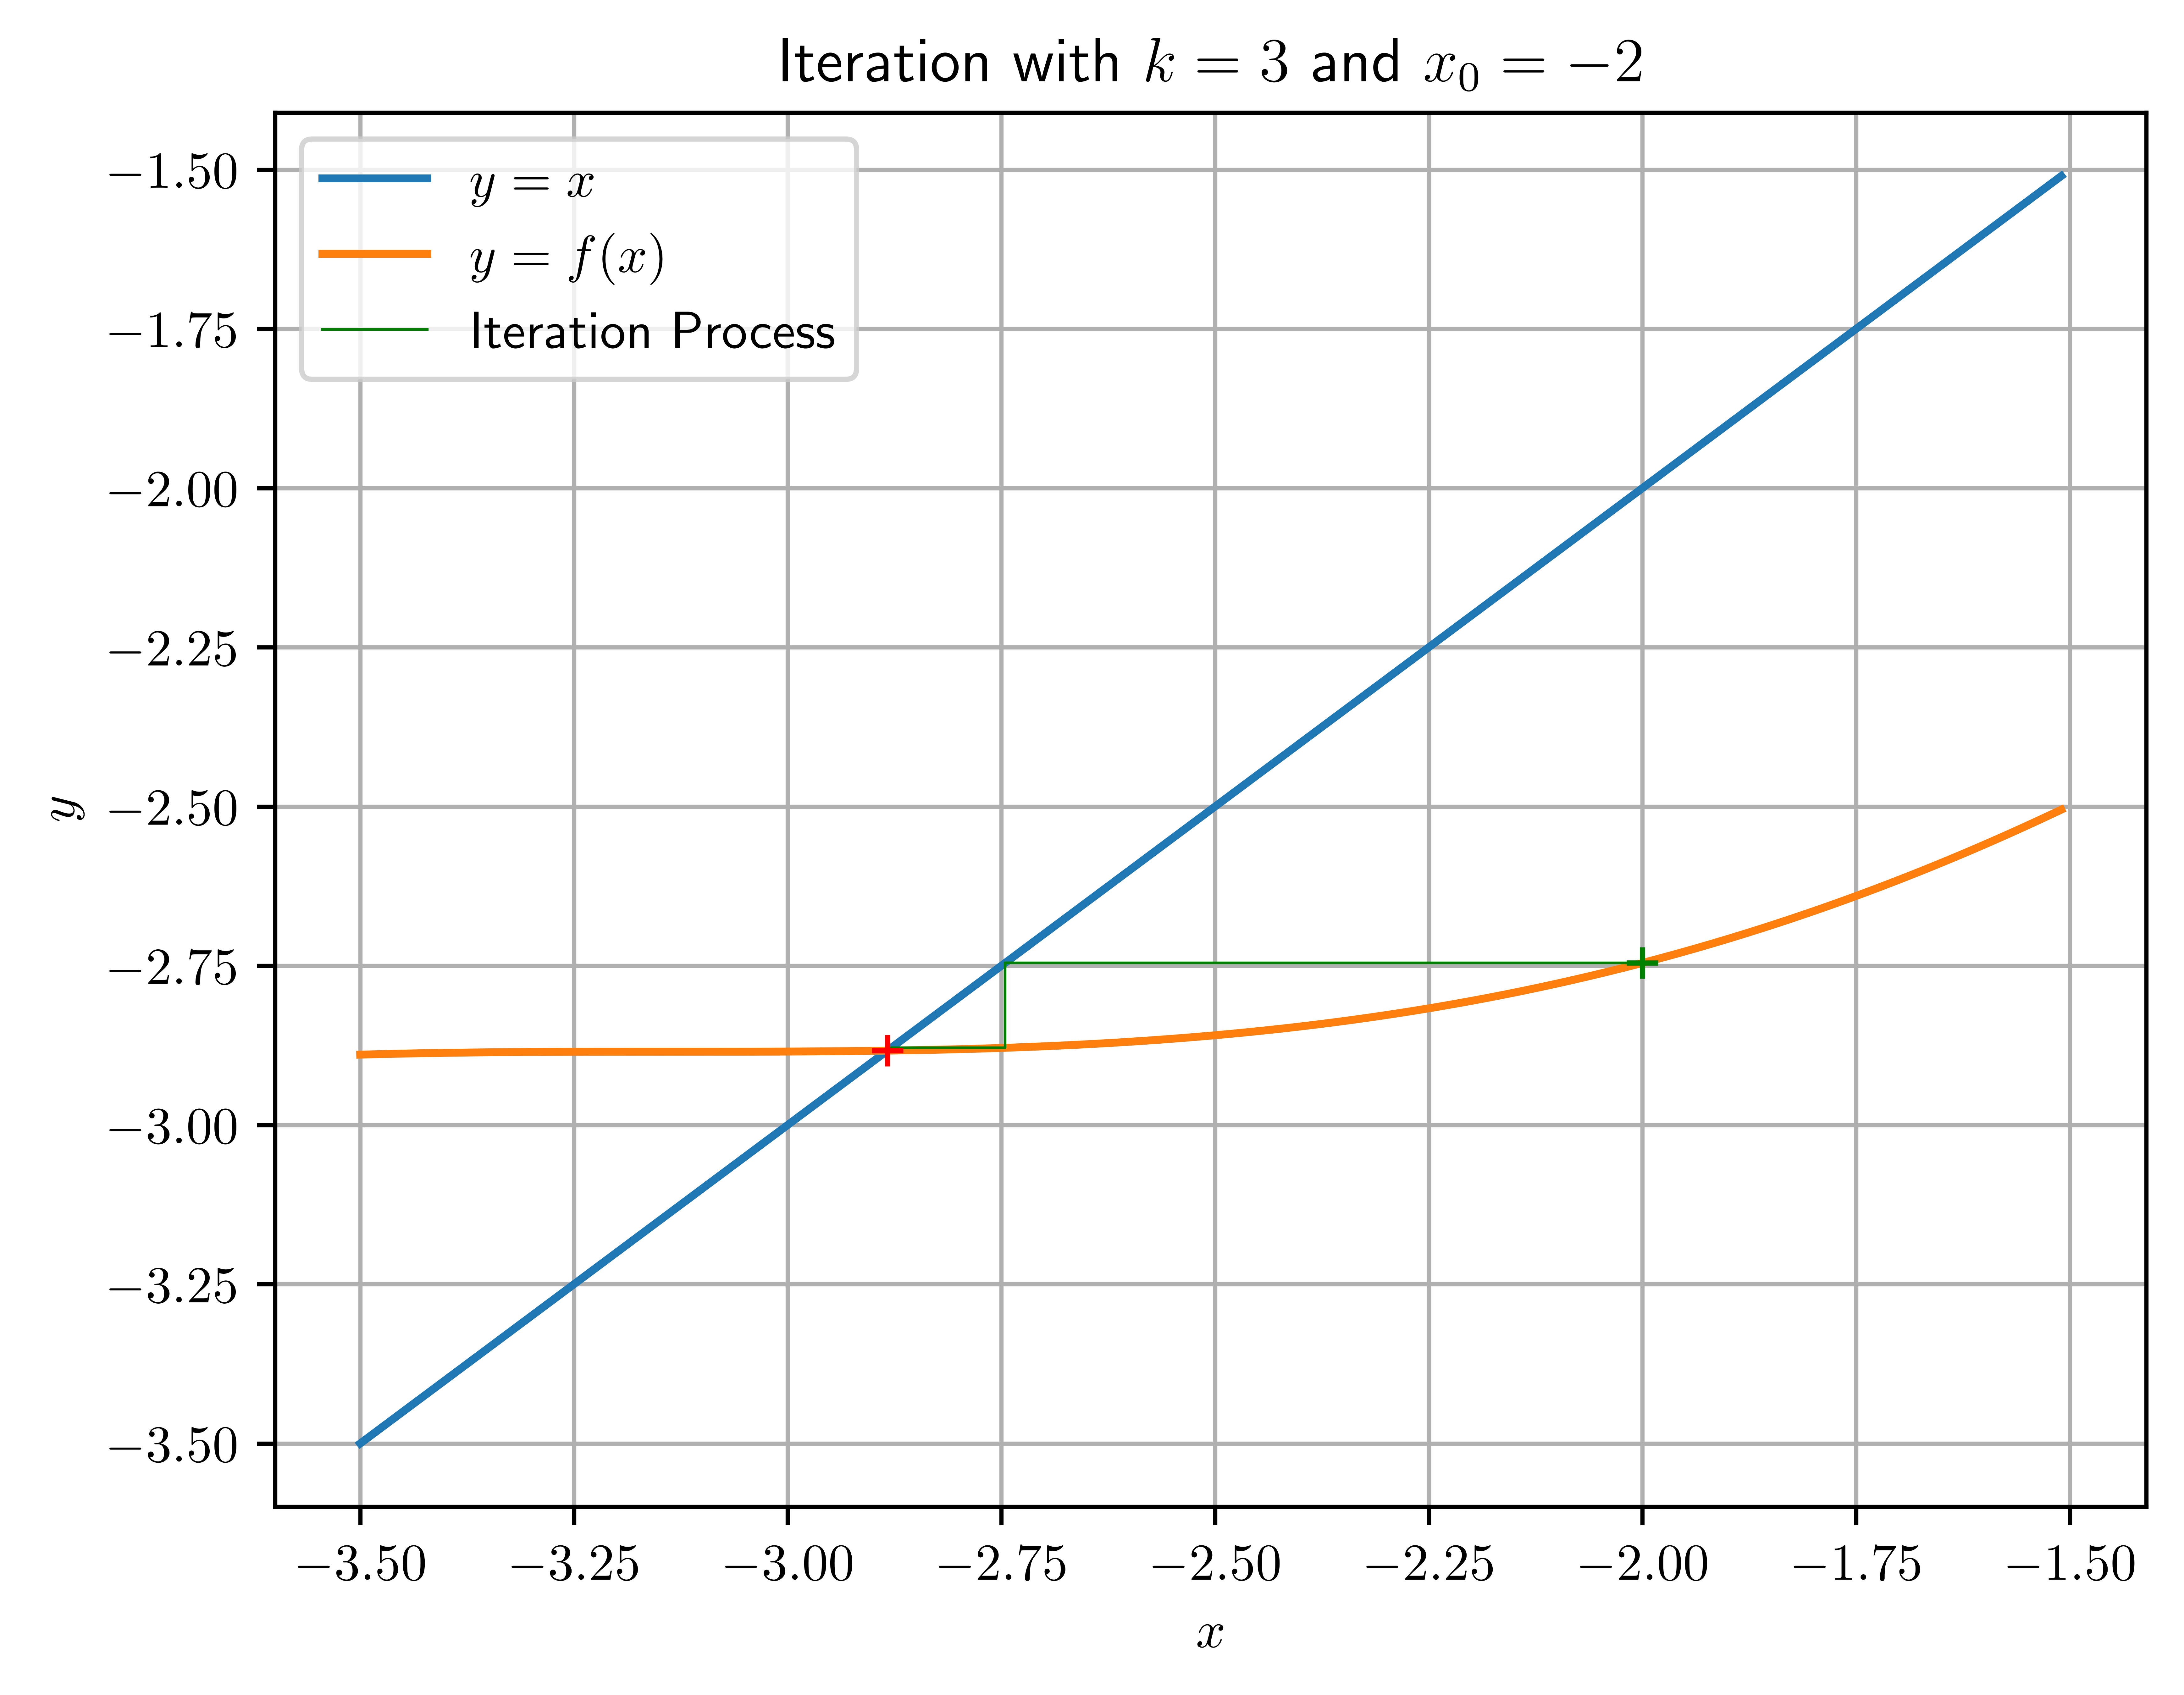
\includegraphics[width=\textwidth]{fig/question-3-iii-1.png}
        \caption{\(k = 3\)}
        \label{fig:question-3-iii-1}%
    \end{subfigure}%
    ~
    \begin{subfigure}[t]{0.5\textwidth}
        \centering
        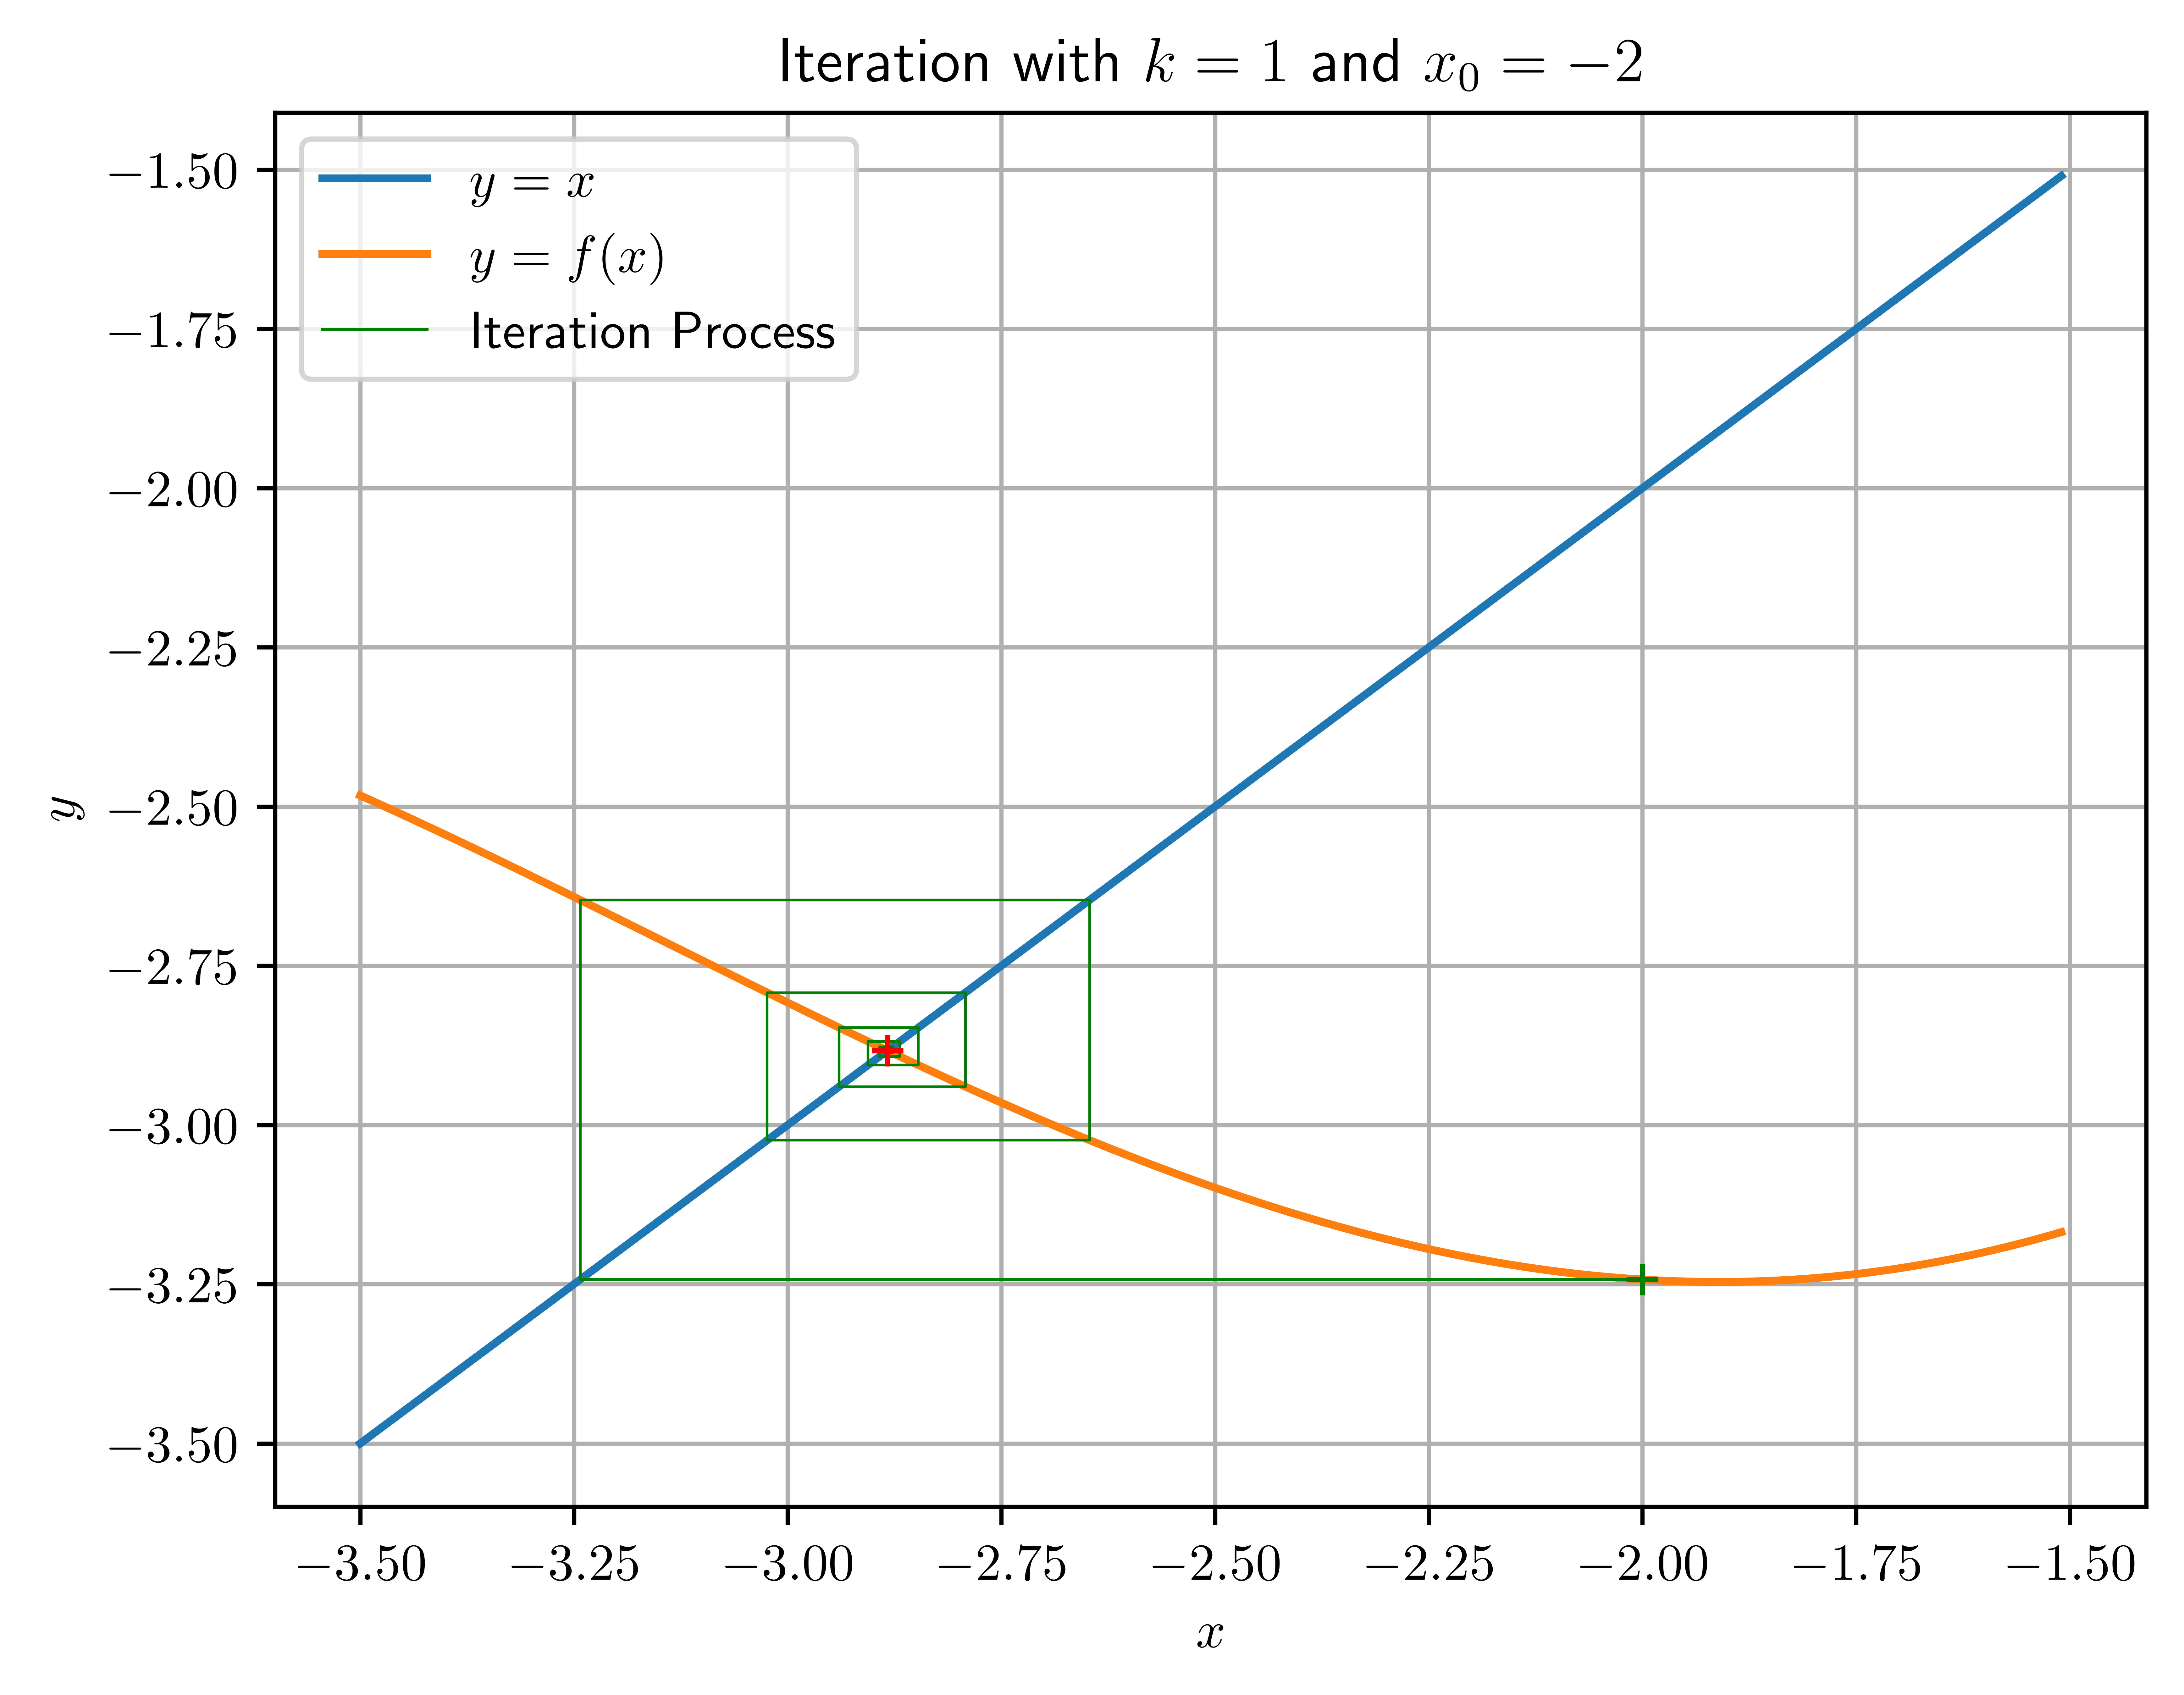
\includegraphics[width=\textwidth]{fig/question-3-iii-2.png}
        \caption{\(k = 1\)}
        \label{fig:question-3-iii-2}%
    \end{subfigure}
    \caption{Oscillatory and Monotonic Iteration Processes with \(x_0 = -2\)}
\end{figure*}

\paragraph{iv. Slow Convergence} By running the code on \(k = 16\), we obtain \autoref{fig:question-3-iv}, terminating after \(N = 34 < 50\) steps. In particular, \(x_{34} = -2.88321\ldots\) and the truncation error \(\epsilon_{34} = \num{2.10845e-5} > \num{1e-5}\).

\begin{figure}[ht!]
    \centering
    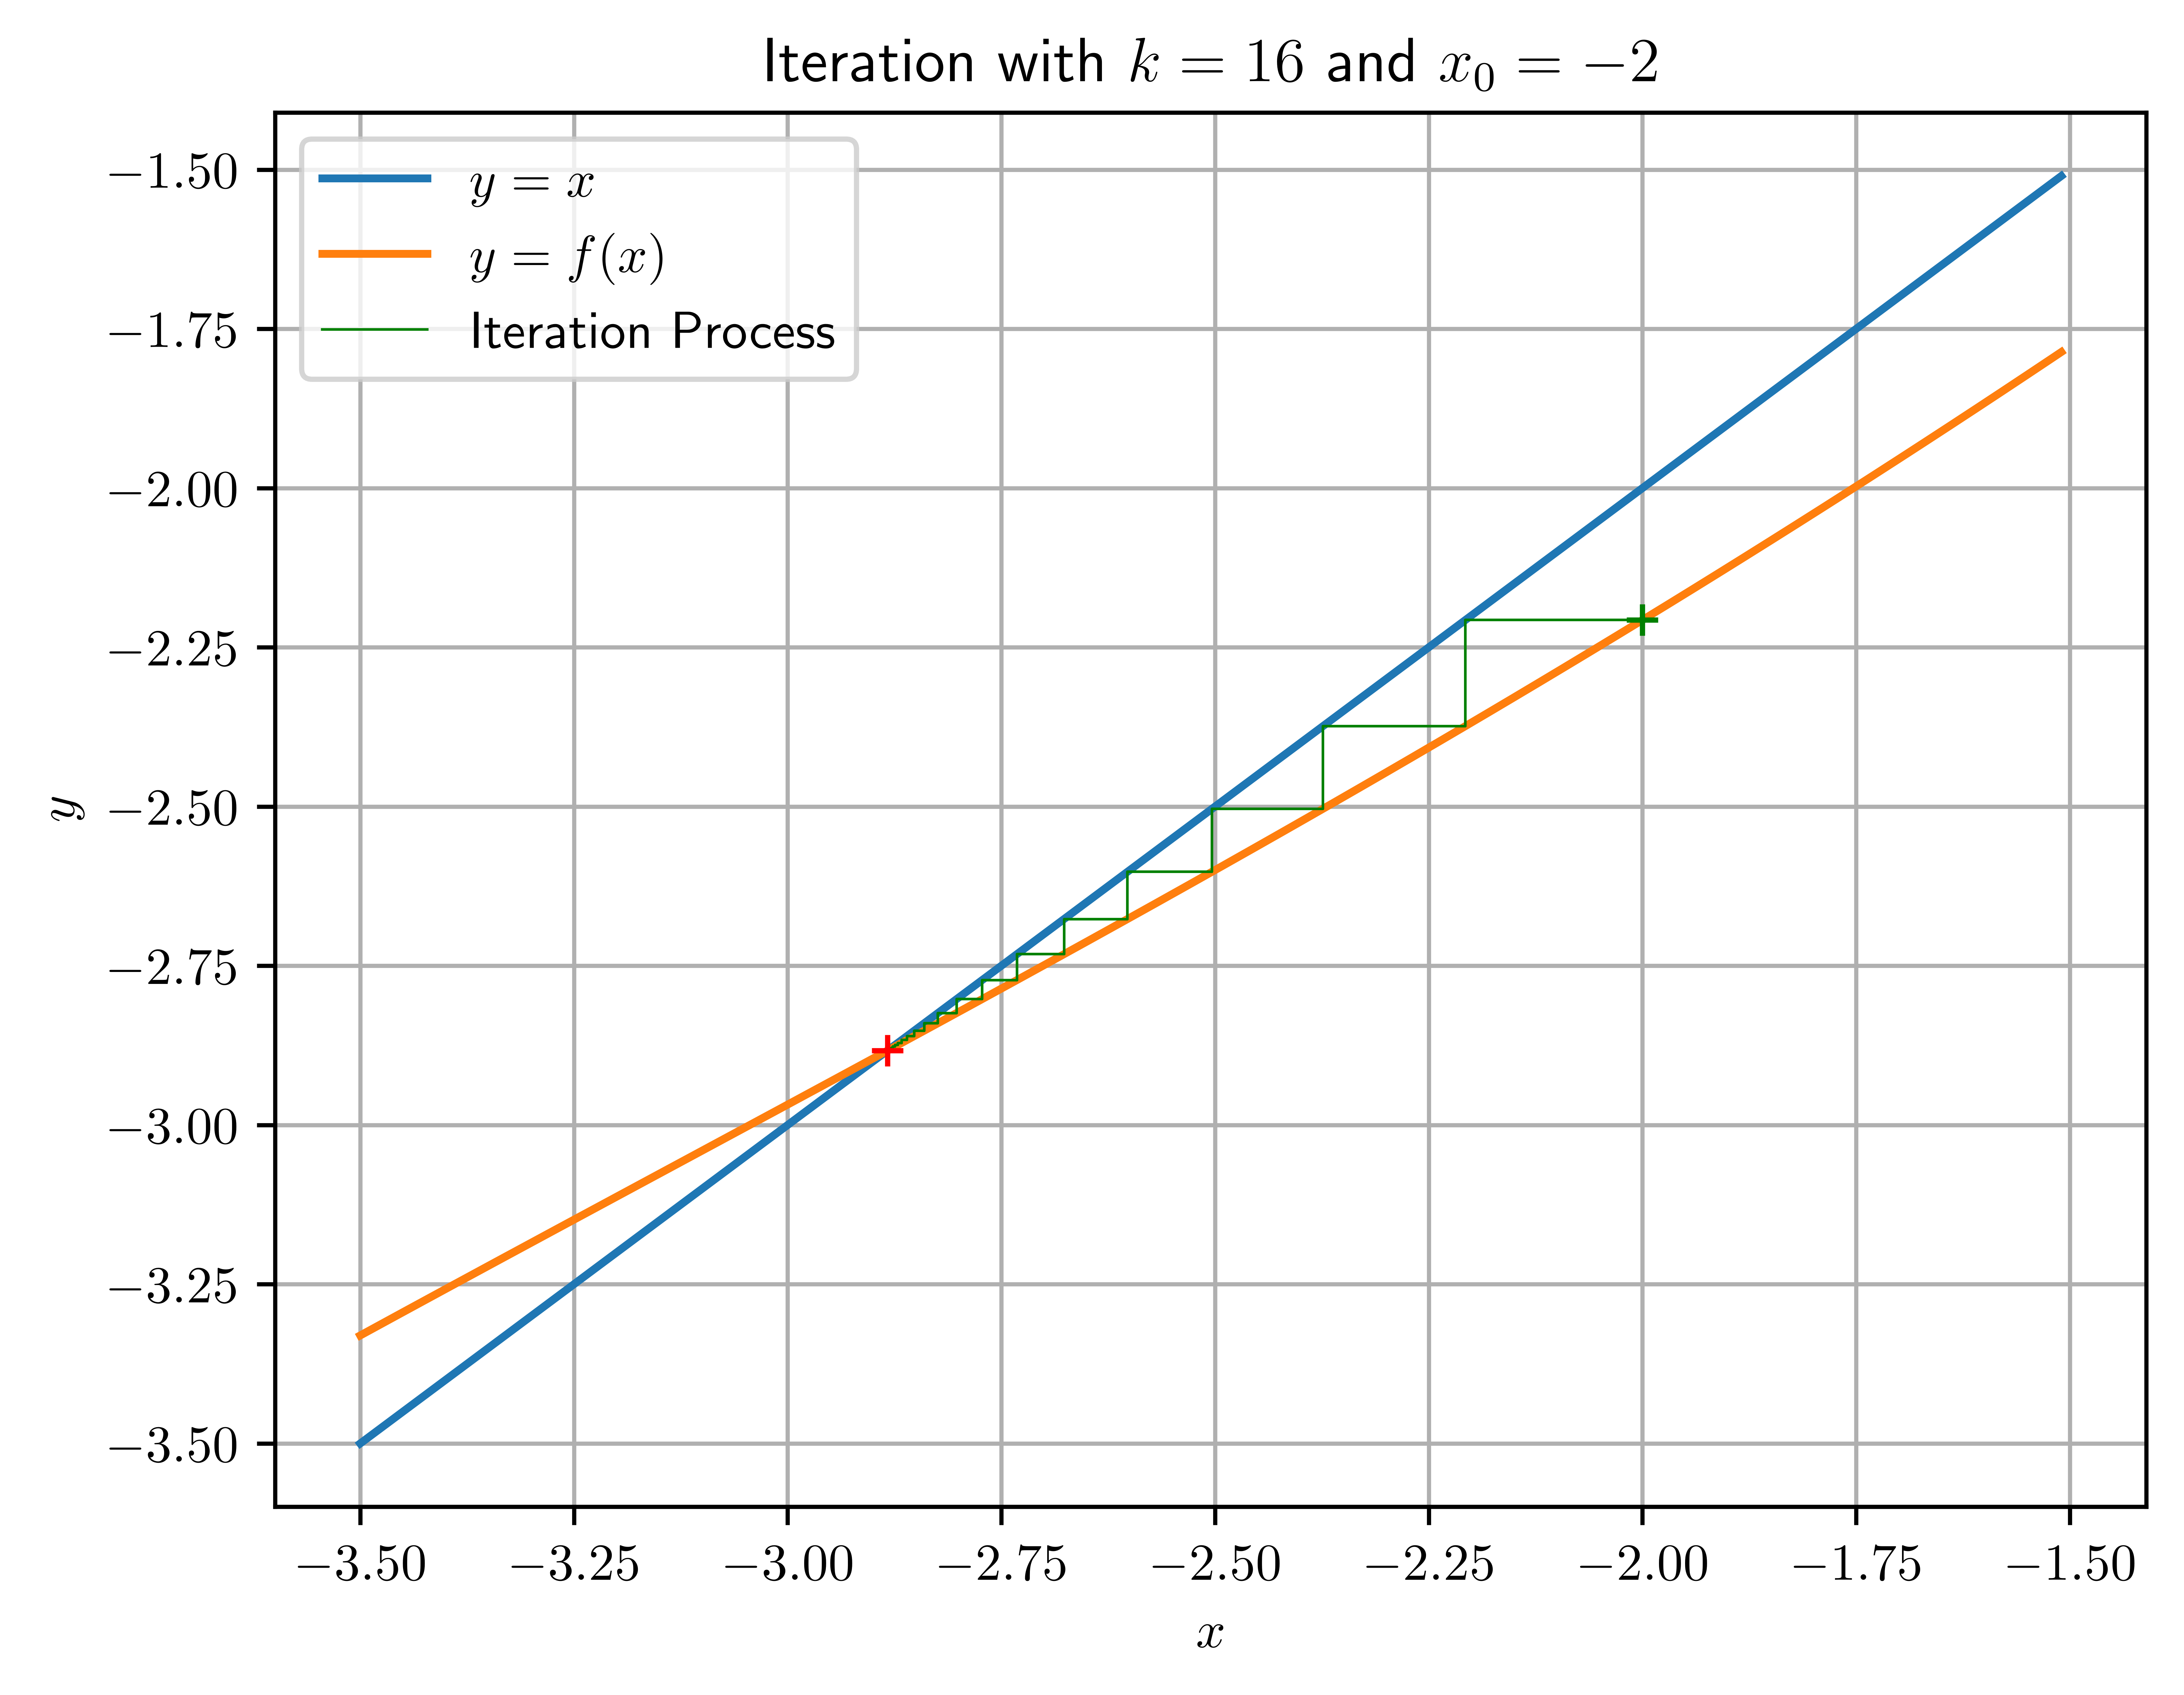
\includegraphics[width=0.8\textwidth]{fig/question-3-iv.png}
    \caption{Iteration Process with \(k = 16\) and \(x_0 = -2\)}
    \label{fig:question-3-iv}%
\end{figure}

We have from \autoref{eq:error-global} that
\begin{equation}
    \abs{\frac{\epsilon_{N + 1}}{\epsilon_{N}}} = \abs{f'\pqty{\xi_N}} \in \ccintv{\inf \abs{f'}}{\sup \abs{f'}}
\end{equation}
where the infimum and supremum is taken between \(x_N\) and \(x_{N + 1}\). Here, we overestimate this interval by taking this over \(\ccintv{-3}{-2}\) (which covers the whole iteration process), hence by numerical calculations,
\begin{equation}
    \ccintv{\inf \abs{f'}}{\sup \abs{f'}} = \ccintv{f'\pqty{-3}}{f'\pqty{-2}} \approx \ccintv{0.72389\ldots}{0.81953\ldots} \subseteq \ccintv{0.72}{0.82}.
\end{equation}

So after \(34\) iterations, using the bound \(\epsilon \in \ccintv{0.75}{1}\), we have
\begin{equation}
    \epsilon_{34} \in \ccintv{0.72^{34} \epsilon_0}{0.82^{34} \epsilon_0} \subseteq \ccintv{0.75 \cdot 0.72^{34}}{1 \cdot 0.82^{34}} \approx \ccintv{\num{1.05770e-5}}{\num{1.11740e-3}}
\end{equation}
and certainly larger than \(\num{1.0e-5}\). This is consistent with our calculation.

\paragraph{v. First-Order Convergence}



\clearpage
\appendix
\section{Listings}

\begin{listing}[htp]
    % \inputminted{python}{src/test.py}
    \caption{Testing Python code}
    \label{lst:example}%
\end{listing}

\end{document}